% =========================================================================
% CHAPTER 3 — LITERATURE AND MARKET REVIEW
% Section 3.1 — Psychological Barriers to Climate Risk Perception
% =========================================================================

\chapter{Literature and Market Review}
\label{ch:literature}

The literature reviewed in this chapter organises around five strands that together define the intersection at which this thesis positions itself: the psychology of climate risk perception, the cognitive science of dynamic and complex systems, the empirical evaluation of climate visualisation, the strands of data humanism, embodied cognition and immersive analytics, and the applications of machine learning to Earth-system science. Each strand is developed as a compact argument rather than as an inventory of publications; the sixth and final section synthesises them into the specific gap the thesis addresses.

% -------------------------------------------------------------------------
\section{Psychological Barriers to Climate Risk Perception}
\label{sec:psych-barriers}

For much of the late twentieth century, the dominant model of climate communication rested on what became known as the information-deficit hypothesis: the assumption that public inaction on climate change reflected a shortage of accurate scientific information, and that closing the knowledge gap would close the action gap. Two decades of empirical research have not been kind to that assumption. \citet{kellstedt2008} showed, in a representative American survey, that respondents who scored higher on climate knowledge expressed \emph{lower} personal concern about the issue and \emph{lower} sense of responsibility for addressing it, an inverse relationship that persisted after controlling for political affiliation and demographic variables. \citet{kahan2015}, extending this line of work, demonstrated that scientific literacy interacted with cultural worldview to \emph{polarise} rather than converge climate attitudes, so that the most scientifically literate members of opposing cultural groups disagreed with each other more sharply than their less-literate counterparts. The uncomfortable finding of this literature is not that information does not matter but that its effects are mediated by cognitive and cultural machinery which the standard formats of climate communication were not designed to address. What has failed is not the messenger's accuracy but the messenger's understanding of who is listening and how.

The most influential systematic account of this failure remains \citet{stoknes2015}, whose typology of five psychological barriers has been widely adopted in the science-communication literature and has structured much of the applied research that followed. The five barriers, which Stoknes labels the \emph{five~Ds}, are \emph{distance} (climate change is perceived as spatially, temporally and socially remote from everyday experience), \emph{doom} (catastrophist framing triggers avoidance rather than engagement), \emph{dissonance} (the gap between climate belief and daily behaviour is resolved by adjusting the belief rather than the behaviour), \emph{denial} (self-protective disengagement from information experienced as threatening) and \emph{identity} (climate positions function as markers of group belonging, making the acceptance of new information contingent on its compatibility with prior identification). The five barriers do not operate independently; \citet{vanderlinden2015} document their interlocking action empirically and argue that effective communication requires addressing them jointly rather than sequentially. The finer-grained segmentation offered by \citet{leiserowitz2021}, in the long-running \emph{Six~Americas} study of the Yale Program on Climate Change Communication, shows that publics stratify into psychologically coherent audiences whose barriers activate differently, so that no single communicative strategy can serve all of them at once. The tempting inference --- that better graphs might solve this --- is not supported by the evidence the following section examines.

The reason conventional visualisation has failed to dissolve the barriers identified by Stoknes and his successors is structural, not aesthetic. \citet{cornerclimate2015}, drawing on empirical work conducted by the Climate Outreach organisation in the United Kingdom, showed that the imagery most frequently used to communicate climate change --- polar bears, smokestacks, calving glaciers, temperature curves --- either reinforces the very psychological distance the communicators hope to close or activates the doom response that suppresses engagement. \citet{nicholsoncole2005}, in what remains a foundational study of the perceptual reception of climate visuals, demonstrated that participants presented with standard scientific climate imagery reported a paradoxical combination of concern and detachment: the imagery made the phenomenon feel real, but it also made it feel finished, already someone else's problem, cognitively closed. The recent review of \citet{ojala2023} synthesises a decade of subsequent work on affective responses to climate communication and concludes that formats which do not offer the reader an active role in relation to the information consistently underperform formats that do. Adding more precision to a line graph does not open such a role; the graph's implicit rhetoric of \emph{here is the fact} leaves the reader with nowhere to stand.

The direction in which the more recent literature has begun to point is towards representational forms that treat the reader as an active participant in the construction of meaning rather than as the passive recipient of an authoritative image \citep{marlon2019, ojala2023}. This shift has taken several forms: narrative-based communication that embeds climate information in stories with which readers can identify \citep{morris2019}, visualisation practices that explicitly invite exploration and interpretation rather than mere reading \citep{cornerclimate2015} and, at the more experimental end, representational practices grounded in embodied and interactive cognition to which this thesis contributes, and which the fourth section of this chapter (§\ref{sec:embodied-viz}) develops in detail. The psychological literature identifies the problem to which the representational literature has yet to find an adequate answer, and the case made in this thesis is that machine learning, treated not as a predictive instrument but as a substrate for representation, offers one path through which that answer might be pursued.

% -------------------------------------------------------------------------
\section{The Cognitive Science of Dynamic and Complex Systems}
\label{sec:cognitive-science}

The psychological literature reviewed in the previous section identified the cultural and affective barriers through which climate information is filtered before it reaches interpretation. The cognitive-science literature reviewed here identifies a barrier of a different kind, prior to filtering and independent of it: the structural limits of the human mind in reasoning about systems whose behaviour is governed by accumulation, feedback and delay. The claim developed in this section is that these limits are not defects of education which better teaching could remedy but stable features of human cognitive architecture, and that any representational strategy which ignores them will fail regardless of how psychologically well-tuned it might be.

The most systematic body of evidence for this claim comes from the work of \citet{sterman2008}, whose two decades of experimental studies have consistently shown that even mathematically literate adults --- graduate students at MIT, engineering professionals, participants with formal training in calculus and dynamics --- make systematic errors when asked to reason about elementary stock-and-flow systems. The experimental design is deceptively simple. Participants were shown a scenario in which atmospheric CO\textsubscript{2} rises gradually and stabilizes at 400~ppmv by 2100 (Figure~\ref{fig:sterman-scenario}), together with the historical trajectory of anthropogenic emissions and the current rate of net removal by oceans and biomass (Figure~\ref{fig:sterman-task}). They were then asked to sketch the emissions path consistent with stabilization. As Figure~\ref{fig:sterman-response} illustrates, 84\% of respondents produced trajectories that violate mass balance: rather than reasoning about the relationship between inflow and outflow, they matched the shape of the output to the shape of the input, keeping emissions well above removal while expecting the stock to stabilize.

% ============================================================
% Sterman (2008) climate stabilization task -- original figures
% extracted from the Science article as vector PDF crops.
%
% Requires the three PDF files in the figures/ folder:
%   sterman_scenario.pdf, sterman_task.pdf, sterman_response.pdf
% (\graphicspath{{figures/}} is already set in main.tex)
% ============================================================

\begin{figure}[htbp]
    \centering
    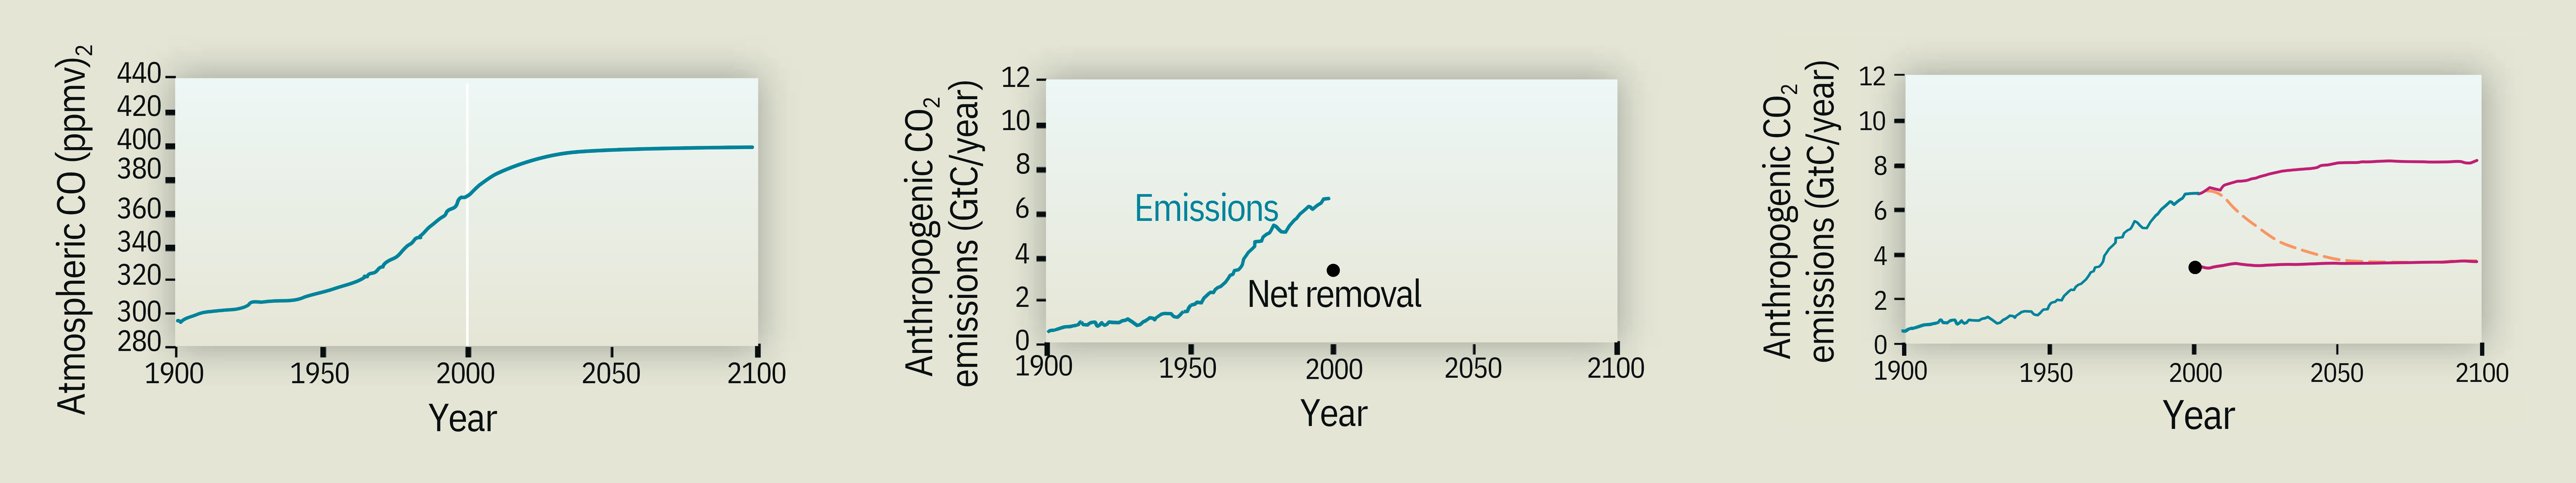
\includegraphics[width=\textwidth]{sterman_panel.png}
    \caption[The climate stabilization task]{The climate stabilization
    task. (a)~The scenario presented to participants: atmospheric
    CO\textsubscript{2} concentration rises gradually to 400~ppmv and
    stabilizes by 2100. (b)~The stock--flow information provided:
    anthropogenic CO\textsubscript{2} emissions from 1900 to 2000 (the
    inflow) and current net removal by oceans and biomass (the
    outflow), with emissions roughly double net removal. (c)~A typical
    response: participants erroneously sketch future emissions that
    match the shape of the CO\textsubscript{2} trajectory
    (pattern-matching heuristic), while mass balance requires emissions
    to fall until they equal net removal (dashed line). Reprinted from
    \citet{sterman2008}.}
    \label{fig:sterman-panel}
\end{figure}

\citet{cronin2009} demonstrated the finding in its starkest form: participants shown a graph of the inflow and outflow of some quantity into a stock were asked to sketch the trajectory of the stock itself, a task equivalent to visually integrating the difference between two curves. Even in scenarios simplified to the point of triviality, the majority produced trajectories that confused rates with levels, mistook peaks in the flow for peaks in the stock and treated the dynamic system as if it were static. The pattern was not distributed randomly across the participant pool; it appeared in the responses of participants who had scored highly on prior tests of mathematical competence and who had, in principle, the technical apparatus to solve the problem correctly. What the study documented was not a failure of arithmetic but a failure of representation --- the mind, given only a graph, does not spontaneously construct the dynamic scenario the graph is meant to depict. The implication for climate communication is direct and uncomfortable: presenting CO\textsubscript{2} emissions and CO\textsubscript{2} concentrations as parallel curves does not communicate that the second is the integral of the first, and readers of the graph will systematically underestimate the inertia of the system \citep{sterman2008}.

A second, converging line of evidence comes from cognitive-load theory as developed by \citet{sweller1988} and extended over three decades of subsequent research \citep{swellervanmerrienboer2019}. The theory rests on a well-documented empirical fact: working memory, the mental resource in which active reasoning occurs, has a strictly limited capacity, and any representational format which requires the reader to hold multiple relationships in working memory simultaneously will produce comprehension errors that scale with the number of relationships. Static visualisations of dynamic systems --- an ensemble spaghetti plot, a set of stacked time series, an isocontour map of projected change --- ask the reader to mentally animate what the visualisation cannot animate directly, to hold in mind the transitions between frames the visualisation cannot show, to construct an internal simulation of a process the graph depicts only in its final state. The cognitive load imposed by this reconstruction is high, and it is imposed \emph{in addition} to the load of understanding the domain itself. The failures of comprehension that result are not deficiencies of the reader; they are predictable consequences of asking working memory to do work for which it does not have capacity. \citet{ware2021}, integrating cognitive-load theory with perceptual research on visual attention, argues that the design of any communicative visualisation must minimise this internal-simulation demand by making the dynamic structure of the system perceptually available in the representation itself.

The third strand of evidence gestures towards the direction in which the following sections will develop. \citet{tversky2019}, in a synthesis of four decades of research on spatial and mental representations, argues that human cognition of complex processes is fundamentally spatial in character: the abstract relationships that constitute a dynamic system are understood through analogy to bodily, spatial and kinaesthetic schemas that the mind already inhabits. This finding is more than a fact about mental imagery; it identifies the cognitive substrate through which any representation of a complex system must be received in order to be understood at all. If systems like the AMOC are structurally dynamic, and human reasoning about dynamic systems is spatially embodied, then the representational strategies most likely to succeed are those which enrol the reader's spatial and kinaesthetic cognition in the reconstruction of the dynamic. This proposition, which the next section develops through the literature on embodied cognition and data physicalisation, is not offered here as a conclusion but as the hypothesis under which the remainder of this chapter is organised.

% -------------------------------------------------------------------------
\section{Empirical Evaluation of Climate Visualisation}
\label{sec:empirical-viz}

The two previous sections established, on the one hand, the psychological and cultural barriers that filter climate information before it reaches interpretation and, on the other hand, the structural limits of cognition that shape what any representation can hope to communicate. This section turns from theory to evidence and asks what has actually been measured about the reception of climate visualisations, and where the resulting empirical literature is thin. The picture that emerges is one of a field methodologically asymmetric: rich in studies of what audiences \emph{prefer} among alternative visualisations and sparse in studies of what audiences actually \emph{understand} when they view them. This asymmetry, more than any single deficit of aesthetics or interactivity, defines the gap this thesis positions itself to address.

The most systematic mapping of the state of the field is offered by \citet{harold2016}, whose review examined the literature on climate-data visualisation against what is known from cognitive and perceptual science about non-expert visual processing. Their central finding is that the standard formats used to communicate climate change --- line graphs of global mean temperature, choropleth maps of projected change, ensemble spaghetti plots, tornado diagrams of sensitivity --- are mismatched to the cognitive resources of the audiences they are meant to inform, and that the mismatch is documented not only in laboratory studies with student participants but in the interpretive errors made by policy audiences with substantial technical training. The finding is corroborated by \citet{mcmahon2015}, whose study of how policy actors interpret IPCC visualisations demonstrated that even trained readers systematically underestimate uncertainty ranges depicted through shaded envelopes and misread ensemble spread as evidence of disagreement rather than as a structural feature of the projection. The specifically visual literature converges with the psychological literature reviewed in §\ref{sec:psych-barriers}: what has failed is not the accuracy of the visualisations but their compatibility with the perceptual machinery through which they are received. \citet{retchless2016}, in a controlled study of alternative encodings for climate uncertainty on choropleth maps, showed that the encodings most commonly used in scientific practice --- bivariate colour schemes and stippled overlays --- produced the poorest comprehension among non-specialist participants, while encodings borrowed from cartographic design traditions performed measurably better. The finding is significant not because it identifies a superior encoding but because it establishes that alternatives exist and that they can be evaluated empirically, a claim which much of the visualisation-design literature makes only in principle.

The more troubling structural finding of the field, however, is what \citet{kause2020} identifies as the persistent gap between preference and comprehension. Their study, one of the few that measured both variables in the same participants, demonstrated that the visualisations participants \emph{preferred} --- those they rated as clearest, most engaging and most trustworthy --- were not the same visualisations that produced the highest measured comprehension of the underlying phenomenon. Participants preferred formats that felt familiar and confident; they understood formats that were structurally aligned with the dynamic being depicted, whether or not they preferred them. A subsequent extension of the work \citep{kause2021} documented the same divergence for the specific case of climate uncertainty, showing that intuitive-seeming icon arrays and confidence bars produced overconfident interpretation while less intuitive but structurally faithful frequency representations produced calibrated interpretation. The methodological consequence is direct and rarely stated: the dominant tradition of preference-based evaluation in the visualisation literature is measuring the wrong variable. Preference is not comprehension, and optimising representations for preference alone risks constructing what \citet{sheppard2015} has called \emph{consoling visualisations} --- images that are received warmly and understood poorly.

The gap in the empirical literature that this thesis addresses can now be stated with precision. Comprehension studies of climate visualisation exist but are outnumbered by preference studies by roughly an order of magnitude, and among the comprehension studies that exist almost none has evaluated experiential or embodied representational formats against conventional graphic ones \citep{harold2016, sheppard2015}. Where comparative studies of alternative formats have been conducted, they have almost always relied on quantitative comprehension tests with population-level inference as their epistemic goal, an approach appropriate for well-defined comprehension outcomes but poorly suited to the exploratory investigation of how non-specialists articulate their understanding of a system for the first time. The methodological space this thesis occupies --- a qualitative, exploratory comparison of three representational conditions using think-aloud protocols and thematic analysis --- is not a replacement for those quantitative traditions but a complement to them, appropriate to a stage of research in which the phenomenon of interest is the \emph{articulation of understanding} itself, and where the depth of interpretive engagement matters more than the breadth of statistical inference \citep{braunclarke2006, smithmcgannon2018}. The evidence base into which this thesis reports is the one identified by the empirical literature as most thinly populated, and it is populated using the methodology the empirical literature identifies as best fit for the question being asked.


% -------------------------------------------------------------------------
\section{Data Humanism, Embodied Cognition and Immersive Analytics}
\label{sec:embodied-viz}

The three previous sections defined the problem this thesis addresses through the successive lenses of psychology, cognitive science and empirical visualisation research. This section turns to the traditions in which the problem's response has begun to take shape. Three related lines of work --- the philosophical account of embodied cognition, the practice of data humanism and physicalisation and the emerging field of immersive analytics --- have converged over the past two decades on a proposition that runs against the mainstream of scientific visualisation: that the intelligibility of complex information depends on the reader's active bodily and perceptual engagement with it, and that representational forms which do not enrol the body and the senses systematically underperform forms that do. Each of the three traditions arrives at this proposition from a different direction, and their convergence provides the theoretical scaffolding on which the design work of Chapter~\ref{ch:translate} is built.

The philosophical grounding of the position was articulated most systematically by \citet{lakoff1999}, whose work on embodied cognition argues that the abstract concepts through which humans reason about complex systems are not disembodied logical structures but extensions of the bodily and spatial experience that human cognition originally evolved to handle. Concepts such as \emph{acceleration}, \emph{feedback}, \emph{stability} and \emph{tipping} are understood, on this view, through the extension of kinaesthetic schemas that the mind has already inhabited --- the sense of a body speeding up, the sense of a movement returning to itself, the sense of a footing that holds, the sense of a footing that gives way. \citet{kirsh2013} provided empirical support for this position in a series of experimental studies showing that participants who were allowed to gesture and move while reasoning about complex processes performed measurably better than participants restricted to inspection of static representations. The finding held across problem types --- mathematical, mechanical and dynamical --- and its consistency has since supported a growing body of design research arguing that representations of complex systems should be understood not as pictures to be viewed but as environments to be inhabited \citep{tversky2019, hurtienne2011}. The implication for climate visualisation is not that graphs should be replaced by simulations but that any visualisation of a system whose reader is expected to reason about dynamic behaviour must offer the reader a form of embodied engagement with the dynamic, whether kinaesthetic, exploratory or perceptual, that inert graphic formats do not provide.

The design tradition that has developed most concretely from this proposition is the practice of \emph{data physicalisation}, defined by \citet{jansen2015} as the construction of physical artefacts whose geometry and material properties encode information for exploration through touch, sight and sometimes sound. The tradition emerged partly in reaction to the perceived limitations of purely visual representation and partly from the design-research community's engagement with tangible interaction \citep{ishii1997}, and it has since produced both craft objects intended for public engagement and rigorous experimental studies comparing physicalisations against equivalent screen-based visualisations. \citet{moere2010} showed, in one of the earliest such comparisons, that participants working with data physicalisations recalled the represented information with greater accuracy and retained it longer than participants working with equivalent bar charts, a finding that has since been extended across data types and modalities \citep{jansen2015}. Parallel to this technical tradition, the practice of \emph{data humanism} associated with the work of Giorgia Lupi \citep{lupi2017} and colleagues at Accurat, Pentagram and Domestic Data Streamers has argued that scientific data communication has been dominated by an aesthetic of dispassionate abstraction that treats the reader as a rational information processor rather than as an embodied and emotional being. The data-humanist alternative --- often executed as hand-drawn or richly illustrated visualisations that foreground authorial voice, imperfection and narrative --- has been received with mixed reactions in the scientific-visualisation literature, but the empirical case for its central claim is stronger than its stylistic surface suggests. Studies of narrative visualisation \citep{segel2010} and of visual explanations grounded in personal experience \citep{morris2019} document consistently that representations which acknowledge the reader as a participant produce measurably deeper engagement than representations that maintain the fiction of a view from nowhere.

The third convergent tradition, more recent and more technically ambitious, is the field of \emph{immersive analytics} as consolidated in the survey volume by \citet{marriott2018}. The field takes as its premise that the immersive display technologies now becoming accessible --- head-mounted virtual reality, augmented reality, large-format wall displays and spatially-aware three-dimensional interfaces --- offer representational affordances that the two-dimensional screen cannot match, and that these affordances are particularly well-suited to data whose structure is inherently spatial, dynamic or multidimensional. Immersive analytics is distinct from earlier scientific visualisation in its explicit orientation towards \emph{analysis by exploration}: rather than presenting a finished view of a dataset, the immersive representation invites the analyst to move through the data, to change viewpoint, to select and to compare, in ways that leverage the same embodied cognitive resources identified by Lakoff and Kirsh \citep{chandler2015}. Empirical evaluations of immersive analytics for scientific data are still limited in number, and the strongest current evidence concerns tasks involving three-dimensional spatial structure and temporal dynamics rather than more abstract representations of complex systems. But the theoretical alignment between immersive analytics and the cognitive-science literature reviewed in §\ref{sec:cognitive-science} is direct, and the practical accessibility of the underlying technologies --- browser-based WebGL for interactive rendering, the Web Audio API for real-time sonification --- has now brought immersive-analytic design within reach of individual research projects at the scale of a Master's thesis. This thesis takes a modest but deliberate step into that space, treating the browser as a medium for embodied representation rather than as a delivery channel for visualisations that could as easily have been printed.

Taken together, the three traditions reviewed in this section support a claim that will structure the remainder of the thesis: the difficulty of communicating complex climate systems to non-specialist audiences is not addressable by refinement within the conventional-visualisation paradigm, and the direction in which the empirical, cognitive and design-research literatures collectively point is one that treats the reader as an active, embodied participant in the construction of understanding. The design of the three representational conditions in Chapter~\ref{ch:translate} is grounded in this claim, and the design decisions made there are defended through the perceptual and cognitive commitments this section has articulated.

% -------------------------------------------------------------------------
\section{Machine Learning for Climate and Earth-System Science}
\label{sec:ml-climate}

The four preceding sections established the representational problem this thesis addresses and the theoretical traditions in which its response is grounded. This section turns to the fifth strand of the literature: the applications of machine learning to climate and Earth-system science, which supply the analytical substrate on which the representational work of Chapter~\ref{ch:translate} is built. The characterisation offered here is not comprehensive; the field is now vast and has been surveyed elsewhere \citep{reichstein2019, sonnewald2021, irrgang2021}. The purpose of this section is more specific: to identify the dominant agenda that has shaped the machine-learning-for-climate literature over the past decade and to locate, against that agenda, the alternative role for machine learning that this thesis undertakes.

The dominant agenda has been broadly \emph{predictive} in orientation. The most cited applications of machine learning to Earth-system data fall into four families: probabilistic short-range forecasting of climate variables through recurrent and convolutional architectures \citep{sonnewald2021, weyn2020}, anomaly detection and event characterisation in observational streams \citep{ham2019}, subgrid-scale parameterisation of physical processes in numerical models \citep{rasp2018, brenowitz2020} and statistical downscaling of coarse-resolution model output to regional scales \citep{vandal2019}. The AMOC-specific literature reflects the same distribution: a growing body of work applies machine-learning techniques to detect early-warning signals in observational and reconstructed transport records \citep{boers2021, ditlevsen2023, benyami2024}, to forecast short-range variability from surface indicators \citep{lu2024} and to identify latent dynamical modes in ensemble reanalyses \citep{sonnewald2019}. The field has developed rapidly, has produced results of substantive scientific value and has established a set of methodological conventions --- benchmark datasets, evaluation protocols and reporting standards --- that are now recognisable across the community. The point relevant here is not that this agenda is misconceived; the point is that it is oriented, almost without exception, toward the production of \emph{new scientific findings for expert audiences}, and that the very success of this orientation has left an adjacent question comparatively unexplored.

The adjacent question concerns what machine learning contributes when the goal is not to produce a new scientific result but to make an existing scientific object \emph{intelligible to non-specialists}. The distinction is worth stating precisely because it is easy to lose. A recurrent neural network trained to forecast the AMOC transport strength six months in advance produces a new quantitative capability, evaluated against a ground-truth held-out record and reported in units --- correlation coefficient, root-mean-square error, calibration score --- that the climate-science community shares. A dimensionality-reduction analysis of the same record produces a latent representation whose value cannot be evaluated in those terms because it does not answer the same kind of question. It answers, instead, a question about \emph{structure}: what are the small number of coordinates that account for most of the record's variability, and what do those coordinates mean physically? The analytical work reported in Chapter~\ref{ch:detect} is of the second kind, and the design work of Chapter~\ref{ch:translate} rests on it. The claim that emerges is not that the AMOC vertical manifold has a novel low-dimensional structure --- the finding is consistent with what oceanographers have understood about the meridional overturning for decades \citep{hannachi2007, buckley2016} --- but that this structure, once recovered and characterised, can serve as the coordinate system through which the AMOC is made available to non-specialist perception. The role of machine learning here is not predictive but \emph{representational}: it produces a substrate on which representational work can be conducted, rather than a forecast whose accuracy is the object of evaluation.

The literature that has treated machine learning in this second, representational role is comparatively thin, but it is not empty. \citet{iten2020}, working in fundamental physics rather than climate science, argued that the latent representations recovered by unsupervised networks can be treated as legitimate epistemological objects --- as ways in which a computational system \emph{proposes} a physical variable that a human interpreter can then examine and name. \citet{camps2019} extended a related argument to seismology, using autoencoder representations of earthquake waveforms as the basis for interactive exploration by non-specialist audiences. In the visualisation-research community, \citet{sacha2018} developed a framework for what they called \emph{visual analytics with machine learning}, in which the model's latent representation is not the final product but the substrate through which the human analyst constructs understanding. The extension of this framework from expert analytics to public communication --- from analyst interfaces to representational artefacts for non-specialists --- has been proposed occasionally in the visualisation literature \citep{munzner2014, cabrera2023} but has been implemented in the climate-communication literature almost nowhere. The specific proposition that this thesis pursues --- that the latent representations recovered from an invisible climate system can be translated into experiential representations legible to non-specialist audiences --- is coherent with the theoretical traditions reviewed in §\ref{sec:embodied-viz} and with the emerging visual-analytics tradition surveyed here, but its systematic empirical development in the climate-communication context has not yet been attempted. The gap this thesis addresses is defined at that intersection.

% -------------------------------------------------------------------------
\section{Synthesis: The Intersection This Thesis Occupies}
\label{sec:literature-synthesis}

Read as a single argument, the five strands of literature reviewed in this chapter converge on a proposition that no single strand articulates on its own. The psychological literature reviewed in §\ref{sec:psych-barriers} establishes that the reception of climate information is filtered through documented cognitive and cultural barriers which conventional formats not only fail to address but occasionally reinforce. The cognitive-science literature reviewed in §\ref{sec:cognitive-science} demonstrates that these barriers are compounded by structural limits on the human capacity to reason about accumulation, feedback and delay from static visual representations. The empirical visualisation research reviewed in §\ref{sec:empirical-viz} documents that the standard formats of climate communication have been evaluated primarily through preference studies rather than through comprehension studies, and that comprehension gains from alternative formats remain largely uncharted. The literatures on embodied cognition, data physicalisation and immersive analytics reviewed in §\ref{sec:embodied-viz} identify the theoretical and design traditions in which the response to this cluster of limitations has begun to take shape, but their application to climate communication has been sporadic and their systematic evaluation on specific climate systems almost absent. The machine-learning-for-climate literature reviewed in §\ref{sec:ml-climate} has developed rapidly and with considerable technical sophistication, but its dominant orientation has been predictive rather than representational, and the possibility that machine-learning-derived latent structures might serve as the coordinate system for perceptually meaningful representation --- rather than as inputs to a forecast --- has not been pursued in the climate context.

The intersection at which these five convergences meet is narrow and empirically unpopulated. It is defined by the combination of five commitments: to a climate system whose invisibility and non-linearity make it a stress-test case for the representational problem \citep{lenton2008, armstrongmckay2022}, to a machine-learning treatment whose purpose is to recover latent structure rather than to forecast outcomes \citep{sonnewald2019, iten2020}, to a design tradition that treats the reader as an embodied and active participant in the construction of meaning \citep{lakoff1999, jansen2015, marriott2018}, to a comparative representational framework in which conventional and experiential formats can be evaluated against one another rather than each on its own terms \citep{harold2016, kause2020} and to a qualitative and exploratory evaluation methodology appropriate to a phenomenon whose measurement is not yet ripe for population-level inference \citep{braunclarke2006, smithmcgannon2018}. No study reviewed in the preceding sections satisfies all five commitments jointly, and the small number of studies that satisfy any three or four of them are distributed across the five disciplinary literatures rather than integrated within a single research programme. The gap this thesis addresses is not the absence of any one of these commitments in the literature; it is the absence of their integration.

The response this thesis makes to the situation identified in the preceding paragraph is deliberately modest in its scope and deliberately specific in its claims. It applies machine learning to the observational and reanalysis records of a single climate system, the Atlantic Meridional Overturning Circulation, in order to recover a latent structure whose faithfulness to the underlying dynamics is defensible on the terms the oceanographic literature itself recognises \citep{hannachi2007, buckley2016}. It designs three representational conditions --- conventional static, interactive dynamic and experiential --- through which that latent structure is translated for non-specialist audiences, and it grounds each design decision in the perceptual and cognitive principles identified in §\ref{sec:embodied-viz}. It evaluates the three conditions through a small-N think-aloud study whose epistemic ambition is the qualitative depth appropriate to a first empirical investigation, not the population-level generalisation that would require a study design outside the scope of this work. The contribution offered is not a novel finding in any of the five literatures reviewed in this chapter but a methodology that connects them, and the case for the value of that methodology rests on the argument that has now been made. The chapters that follow are its execution.